\documentclass[aspectratio=169]{beamer}
\usepackage[T1]{fontenc}
\usepackage[default]{sourcesanspro}
\usepackage{newtxsf}
\usepackage{hyperref}
\usepackage{latexsym,amsmath,xcolor,multicol,booktabs,calligra}
\usepackage{graphicx,pstricks,listings,stackengine}
\graphicspath{{./figures/}}
\usepackage{lipsum}
\usepackage{wrapfig}
\usepackage{url}
\usepackage{subcaption}
\usepackage{listings}
\usepackage{minted}
\setminted{fontsize=\footnotesize}
\usepackage{fontawesome5}

\usepackage{etoolbox}

\author{Yan Lin}
\title{AI Systems \& Infrastructure}
\subtitle{Module B.4: Cloud Deployment}
\institute{%
    \href{https://www.yanlincs.com}{www.yanlincs.com}
}
\date{September 1st, 2026}
\usepackage{AAU}
\AtBeginSubsection{}
\setbeamertemplate{navigation symbols}{}

\def\cmd#1{\texttt{\color{red}\footnotesize $\backslash$#1}}
\def\env#1{\texttt{\color{blue}\footnotesize #1}}
\definecolor{aauyellow}{RGB}{167, 131, 55}
\definecolor{aaublue}{RGB}{32, 26, 78}
\definecolor{aaured}{RGB}{152, 43, 28}
\definecolor{textgrey}{RGB}{60, 60, 60}

\setbeamercolor{normal text}{fg=textgrey}
\usebeamercolor[fg]{normal text}

\def\emphasis#1{{\color{aaured}\textbf{#1}}}
\renewcommand{\thefootnote}{}


\lstset{%
    basicstyle=\ttfamily\small,
    keywordstyle=\bfseries\color{deepblue},
    emphstyle=\ttfamily\color{deepred},
    stringstyle=\color{deepgreen},
    numbers=left,
    numberstyle=\small\color{halfgray},
    rulesepcolor=\color{red!20!green!20!blue!20},
    frame=shadowbox,
}

\begin{document}

\begin{frame}[plain,noframenumbering]
    \titlepage
    \vspace*{-0.6cm}
    \begin{figure}[htpb]
        \begin{center}
            
\includegraphics[keepaspectratio, scale=0.5]{aau-logo-left-uk}
        \end{center}
    \end{figure}
\end{frame}

\begin{frame}
\tableofcontents[sectionstyle=show,
subsectionstyle=show/shaded/hide,
subsubsectionstyle=show/shaded/hide]
\end{frame}


\section{Whose Machine Runs the Container}

\begin{frame}{Recap: where we are}
    In Module B.3 we packaged our AI API server into a container image that anyone with Docker can pull and run.

    That solves the \textit{how do we ship the software} problem.
    It leaves the \textit{whose machine does it run on} problem wide open.
\end{frame}

\begin{frame}{Our laptop is not the answer}
    Running the container on our laptop is fine for development.
    As soon as we want anyone else to use the API, our laptop becomes a bad host.

    \begin{itemize}
        \item We probably do not want it powered on 24/7
        \item Our home electricity and internet connection might not be reliable
        \item The moment the laptop goes to sleep, the API stops responding
    \end{itemize}

    \vspace{0.5em}
    The standard answer: rent a computer somewhere else, and run our container there.
\end{frame}


\section{What Is the Cloud}

\begin{frame}{Other people's computers}
    \begin{figure}[htpb]
        \begin{center}
            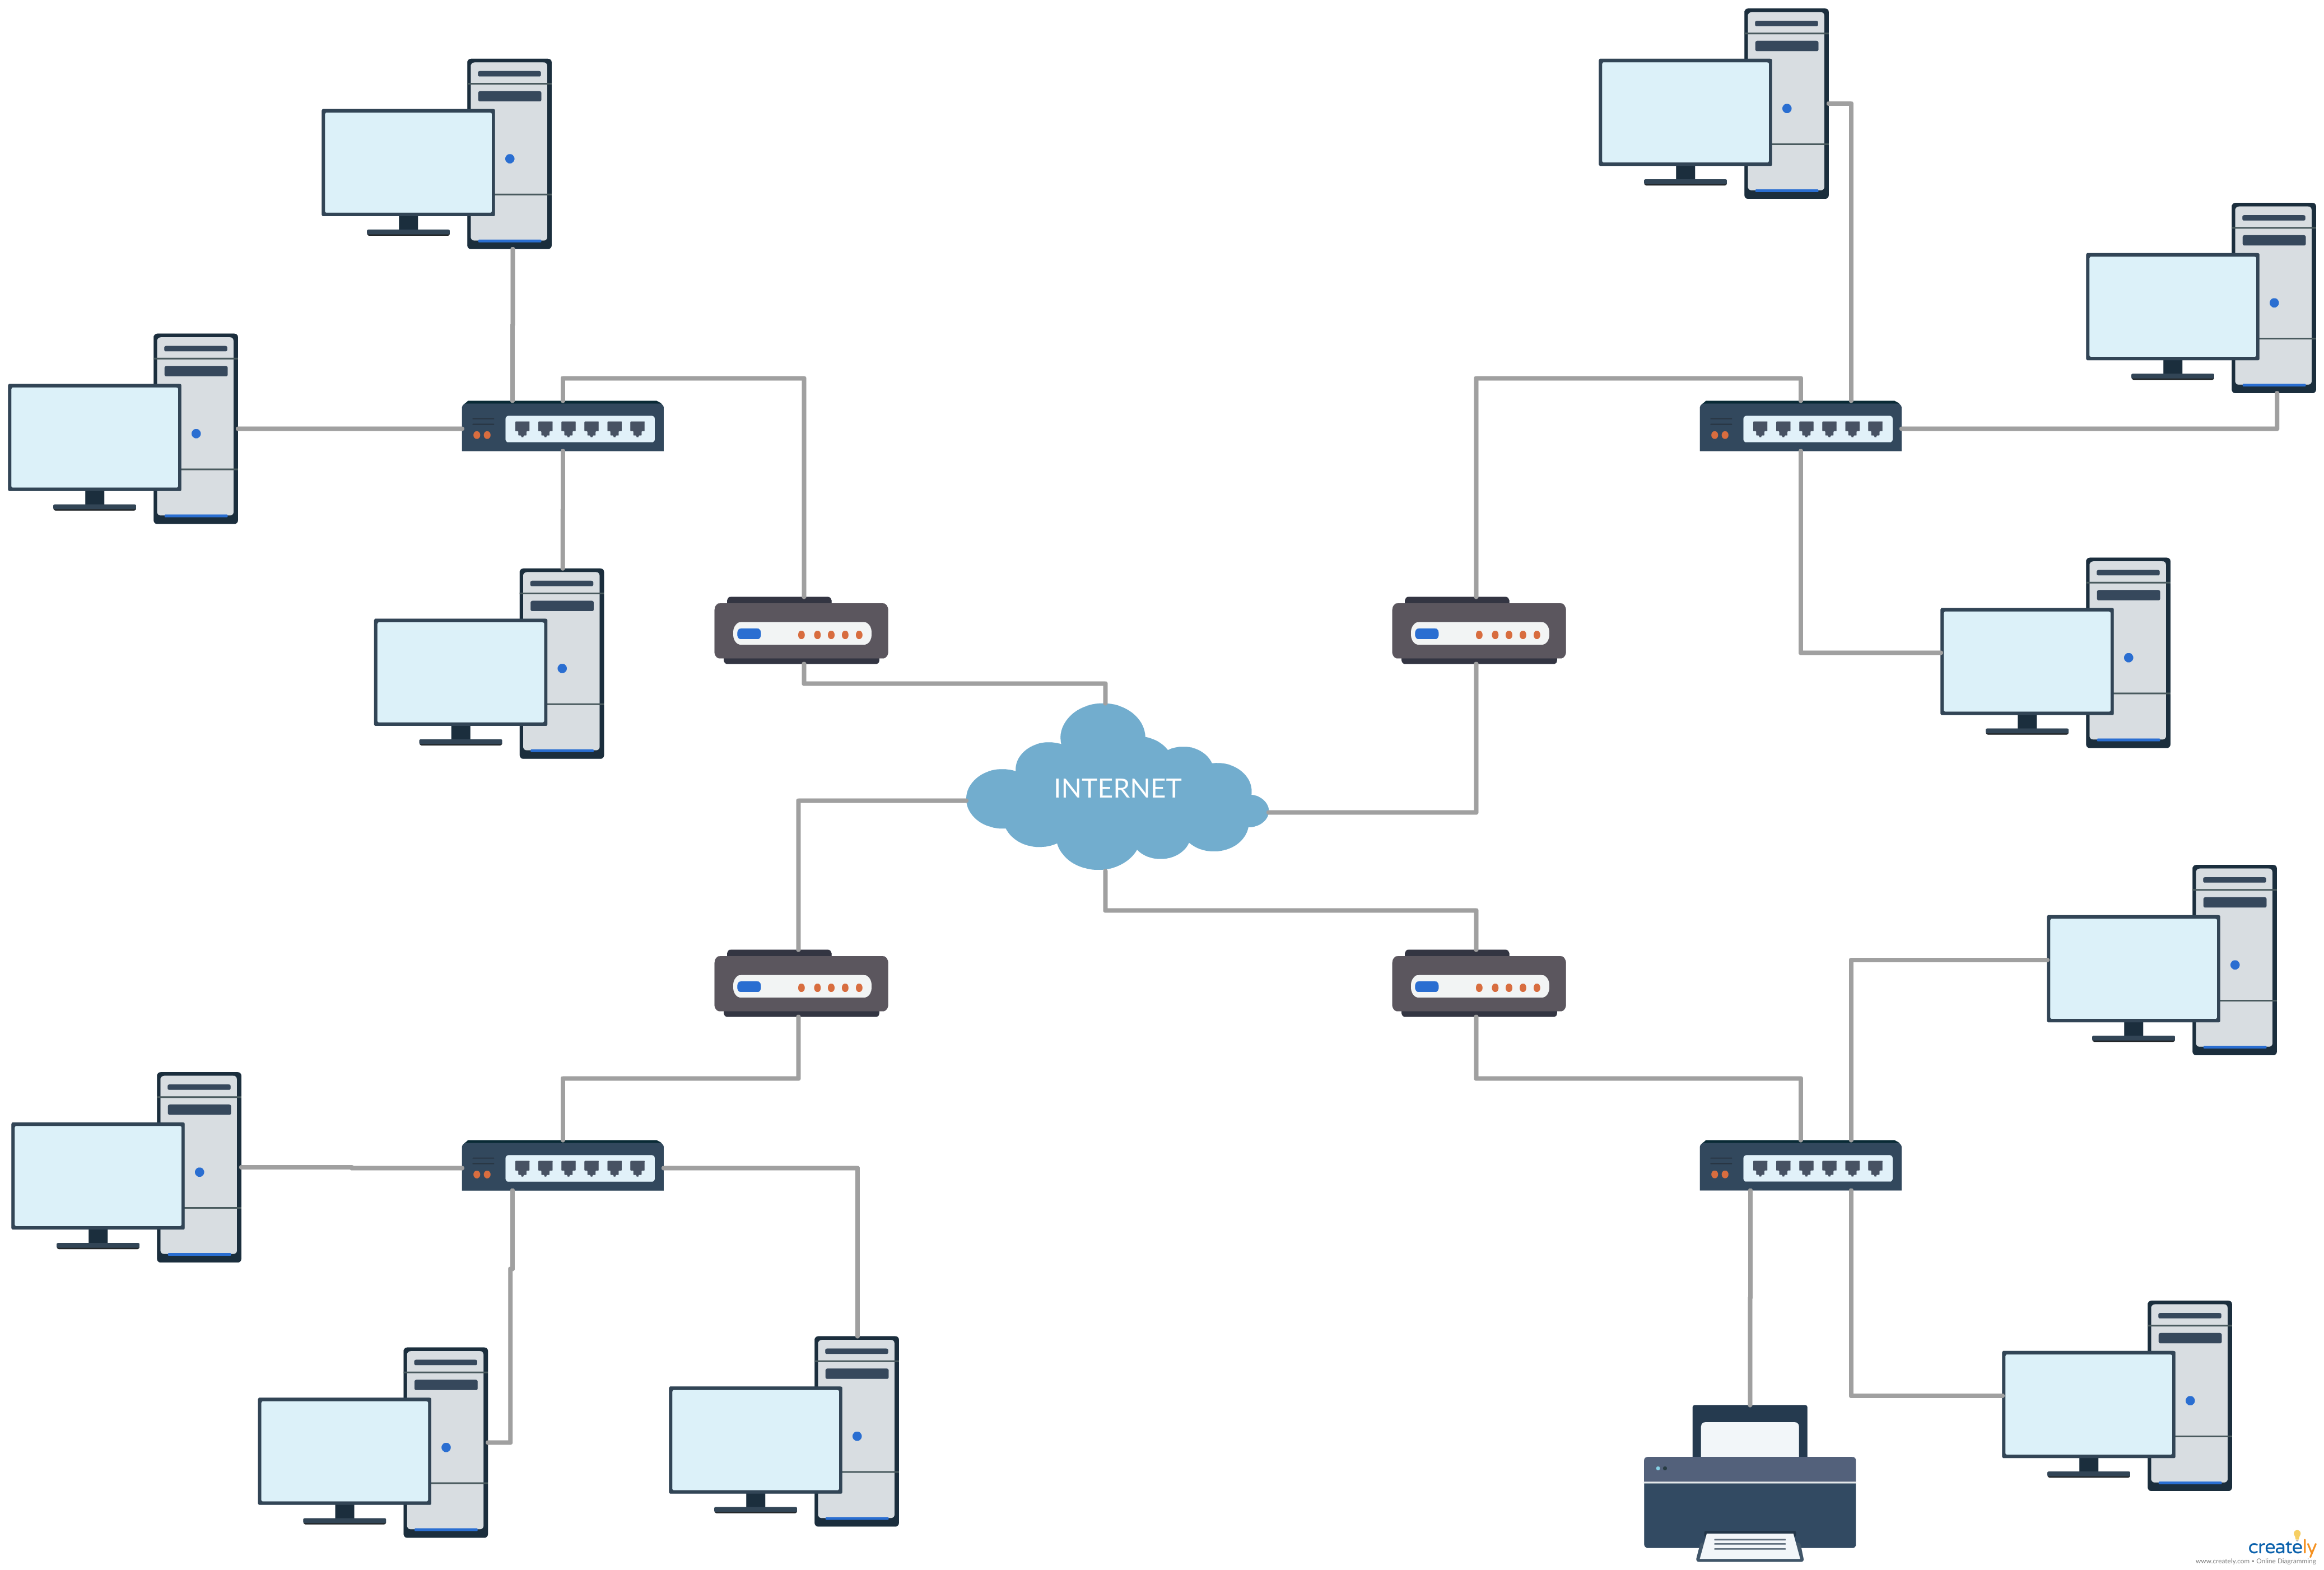
\includegraphics[width=0.45\textwidth]{network_cloud_diagram}
        \end{center}
    \end{figure}

    Not a new kind of computing or a special technology.
    The cloud is other people's computers, sitting in data centers, that we rent over the internet.
\end{frame}

\begin{frame}{Why the cloud exists}
    Around 2006, Amazon noticed that the infrastructure they had to size for peak shopping load sat idle most of the time.
    That idle capacity could be rented to other people who would otherwise have to buy their own servers.

    \begin{block}{For us as customers}
        \begin{itemize}
            \item A new computer ready in minutes instead of weeks
            \item Pay for what we use rather than buying hardware up front
            \item Someone else worries about hardware failures, electricity, and network
        \end{itemize}
    \end{block}

    \begin{block}{The downside}
        We are now dependent on the provider's pricing, availability, and policies.
    \end{block}
\end{frame}

\begin{frame}{Virtualization, the technical trick}
    A single physical server in a data center is a powerful machine, often with dozens of cores and hundreds of gigabytes of RAM, far more than most small customer needs.

    \begin{figure}[htpb]
        \begin{center}
            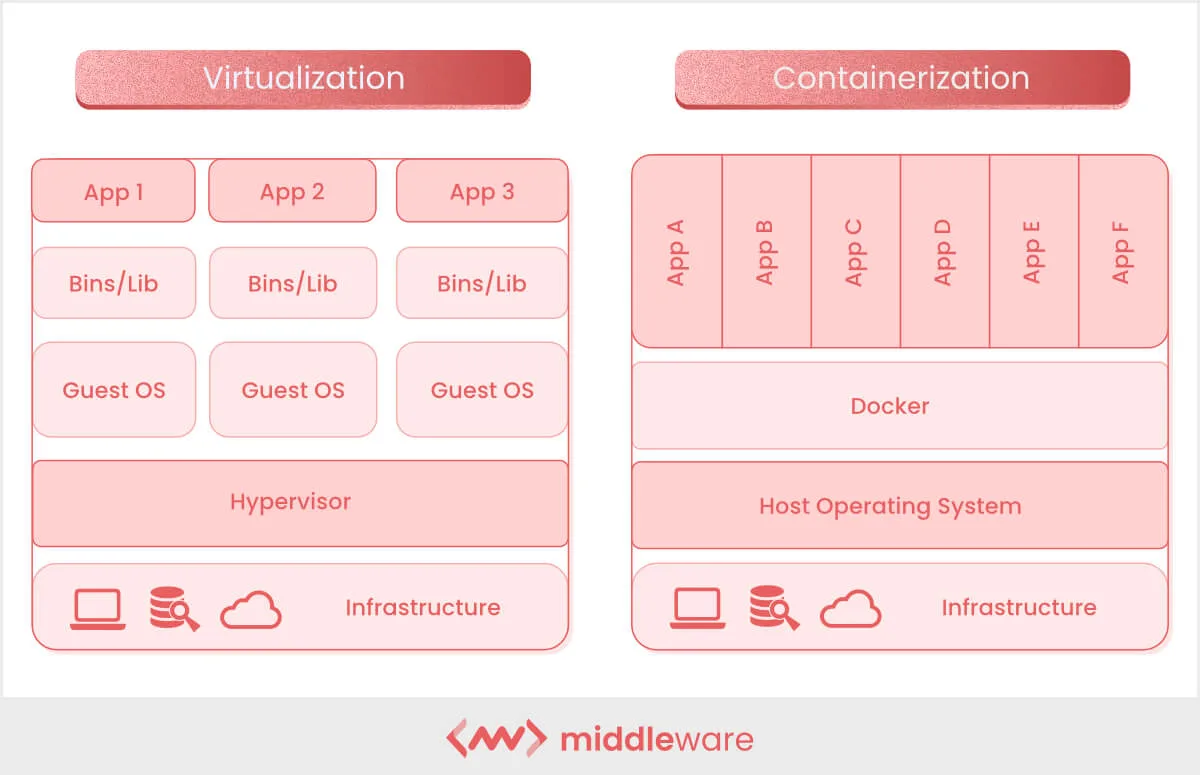
\includegraphics[width=0.45\textwidth]{virtualization}
        \end{center}
    \end{figure}

    Virtualization lets the provider slice that machine into many smaller \textbf{virtual machines} through a small piece of software called a hypervisor.
    Each VM behaves like a complete computer with its own CPU, memory, disk, and OS.
\end{frame}

\begin{frame}{Containers and VMs, side by side}
    We met containers in Module B.2 with the same kind of diagram. Both provide isolation, at different levels.

    \begin{block}{VM}
        Virtualizes the entire hardware and runs its own kernel.
        Can run a completely different OS from the host.
    \end{block}

    \begin{block}{Container}
        Shares the host's kernel and only ships userspace files.
        Lighter, but the host kernel ultimately decides what is allowed.
    \end{block}

    In practice cloud providers rely on both: the hypervisor splits each physical server into VMs sold to different customers, and inside each VM the customer typically runs containers to package and deploy applications.
\end{frame}

\begin{frame}{The big three and the rest}
    \begin{block}{Hyperscalers}
        \begin{itemize}
            \item AWS: the original, biggest catalog
            \item GCP: focus on data and ML services, competitive GPU pricing
            \item Azure: natural fit for the Microsoft ecosystem
        \end{itemize}
    \end{block}

    \begin{block}{Smaller providers, often a better fit for individuals}
        \begin{itemize}
            \item DigitalOcean, Linode, Vultr: clean UIs, predictable pricing
            \item Lambda, CoreWeave, RunPod: GPU rentals at lower prices
            \item Hetzner, OVHcloud, Scaleway: EU-based, often cheap basic VMs
        \end{itemize}
    \end{block}

    \vspace{0.3em}
    For this course it does not matter which one. The recipe (rent a VM, install Docker, run your container) translates across all of them.
\end{frame}


\section{Common Cloud Services}

\begin{frame}{Three categories that matter for us}
    \begin{block}{Virtual machines}
        A rented VM we can SSH into and treat as our own server.
        We install whatever we want, get charged per hour the VM is running.
        EC2, Compute Engine, Azure VMs.
    \end{block}

    \begin{block}{Container services}
        The provider runs our Docker container without us managing the underlying VM, often with autoscaling.
        ECS, Cloud Run, Container Apps.
    \end{block}

    \begin{block}{GPU instances}
        VMs with one or more GPUs attached, for training models or running inference on heavier ones.
        Powerful but among the most expensive line items.
    \end{block}
\end{frame}

\begin{frame}{Why start with a plain VM}
    A reasonable first instinct when browsing a cloud catalog is to reach for the most automated option.
    For learning and small AI services, we argue the opposite is usually wiser.

    \begin{block}{Predictable cost}
        A small VM rents at a fixed hourly or monthly rate, regardless of traffic.
        Usage-based services have produced six-figure bills from static sites, four-figure S3 charges from scraped buckets, GPU instances left running through the weekend.
    \end{block}

    \begin{block}{Transparency}
        On a VM we install Docker ourselves, run our container with \texttt{docker run}, and when something breaks we can SSH in and check \texttt{docker logs}.
        Managed services tend to wrap our app in their own scheduling, networking, and logging layers.
    \end{block}
\end{frame}


\section{Deploying to a Cloud VM}

\begin{frame}{The flow is always the same}
\begin{minipage}[t]{0.4\textwidth}
    Every provider has a slightly different web console, but the deployment flow is always the same.

    \begin{enumerate}
        \item Create a VM
        \item SSH in
        \item Install Docker
        \item Run the container
    \end{enumerate}
\end{minipage}
\hfill
\begin{minipage}[t]{0.58\textwidth}
    \begin{figure}[htpb]
        \begin{center}
            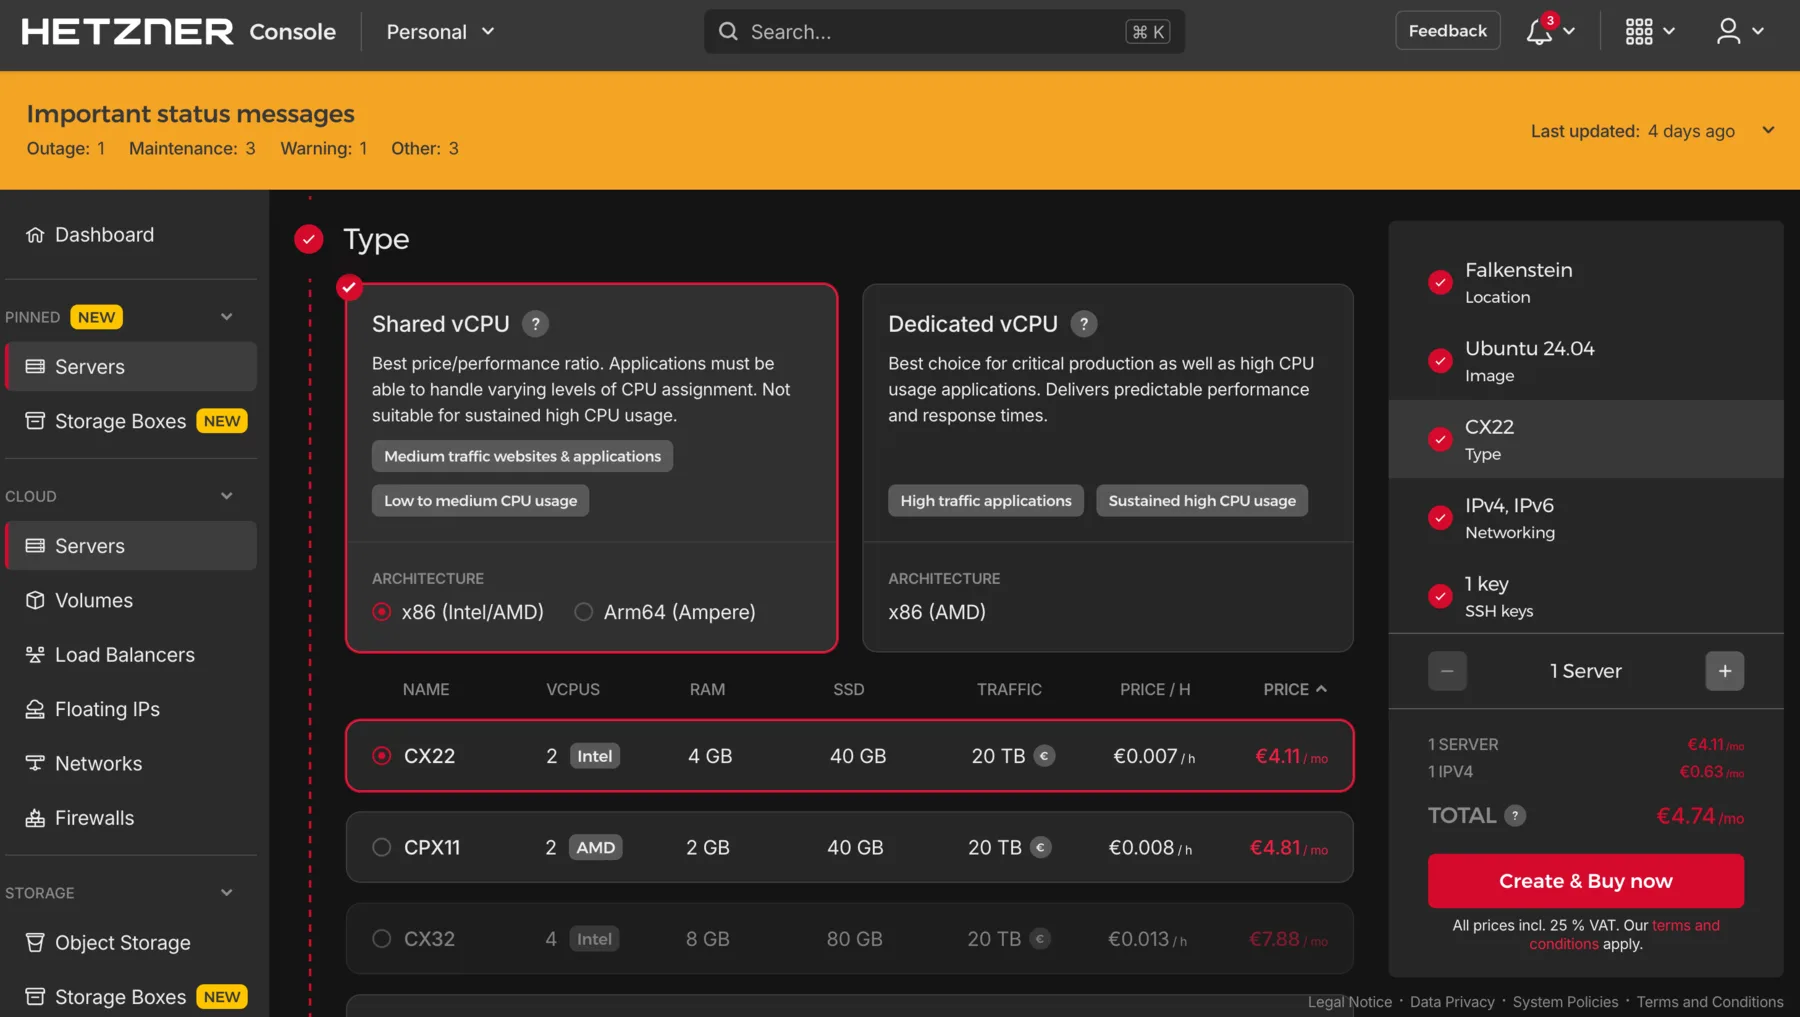
\includegraphics[width=1.0\textwidth]{vm-creation}
        \end{center}
    \end{figure}
\end{minipage}
\end{frame}


\begin{frame}[fragile]{Once the VM boots}
    SSH in, install Docker following the official guide.
    Then run the container.

    \begin{minted}{bash}
docker run -d --name ai-server \
    -p 8000:8000 \
    --restart unless-stopped \
    yourusername/my-ai-server:1.0
    \end{minted}

    \texttt{--restart unless-stopped} brings the container back up after crashes or VM reboots.

    Then, from your laptop:
    \begin{minted}{bash}
curl http://<vm-ip>:8000
    \end{minted}
\end{frame}


\section{Going Public}

\begin{frame}{What is still missing}
    The container is now reachable at \texttt{http://<vm-ip>:8000}, which is technically a working public AI service but almost no one would actually use.

    \begin{itemize}
        \item An IP is not how most people find things on the internet. Hard to remember, and fragile when the VM changes
        \item Plain HTTP traffic is unencrypted. Any network in between can read and modify it
        \item Modern browsers increasingly refuse to talk to non-HTTPS endpoints
    \end{itemize}

    \vspace{0.5em}
The fix is to have a \textbf{domain name} and an \textbf{HTTPS certificate}.
\end{frame}

\begin{frame}[fragile]{Domains and DNS}
    Recall from Module A.1: domain points to one or more IP addresses.
    The Domain Name System turns names into addresses.

    We need an \textbf{A record} mapping our domain to our VM's IP.
    \begin{minted}{text}
api.example.com.   A   <vm-ip>
    \end{minted}

    \begin{block}{Where to get a domain}
        \begin{itemize}
            \item DuckDNS: free subdomain like \texttt{myaiapi.duckdns.org}
            \item Registrars (Cloudflare, Porkbun, Namecheap): own domain, 10-15 EUR per year for a typical \texttt{.com}
        \end{itemize}
    \end{block}
\end{frame}

\begin{frame}{Why HTTPS}
    HTTPS (HTTP over TLS) wraps HTTP in an encrypted, authenticated tunnel.
    \begin{itemize}
        \item Encrypts traffic so a network observer sees only scrambled data, only the sender and the receiver can decrypt the data
        \item Lets the client verify it is talking to the real \texttt{api.example.com} via a certificate
    \end{itemize}

    Since 2015, \textbf{Let's Encrypt} issues free, automated certificates, valid 90 days and renewable indefinitely.
\end{frame}

\begin{frame}{Reverse proxy in front of the container}
    Our containerized server speaks plain HTTP on port 8000, and we are not going to teach it HTTPS directly.

    \begin{figure}[htpb]
        \begin{center}
            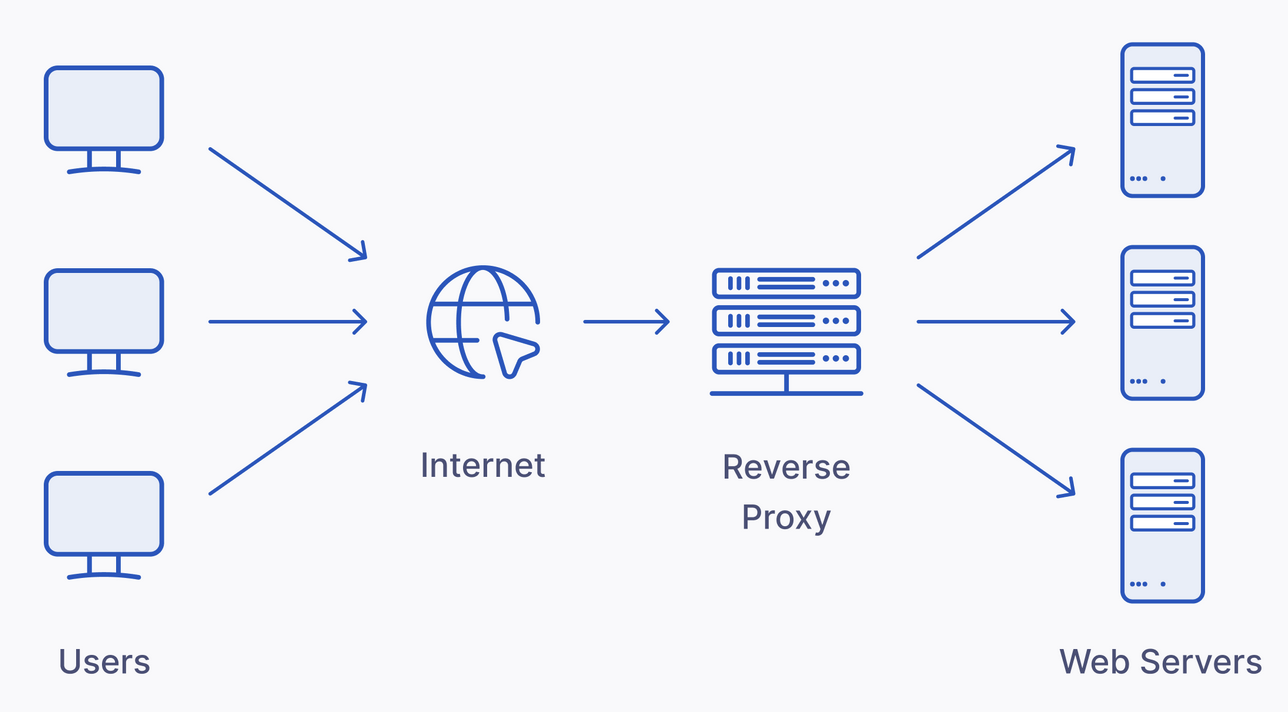
\includegraphics[width=0.5\textwidth]{reverse_proxy_diagram}
        \end{center}
    \end{figure}

    The standard pattern is to put a \textbf{reverse proxy} in front: a separate program that listens on ports 80 and 443, terminates HTTPS, and forwards the decrypted request to our container.
\end{frame}

\begin{frame}[fragile]{Nginx}
    The most common reverse proxy. Small and fast, around since 2004.

    \begin{itemize}
        \item A single Nginx instance handles tens of thousands of simultaneous connections on modest hardware
        \item Functionalities beyond HTTPS termination: access logs, rate limits, caching, compression, load balancing, serving static files
    \end{itemize}

    \begin{block}{Install on Ubuntu}
        \begin{minted}{bash}
sudo apt install -y nginx
        \end{minted}
        Starts automatically, serves a default welcome page on port 80.
    \end{block}
\end{frame}

\begin{frame}[fragile]{Minimal Nginx config}
    Create \texttt{/etc/nginx/sites-available/api.example.com}:
    \begin{minted}{nginx}
server {
    listen 80;
    server_name api.example.com;

    location / {
        proxy_pass http://127.0.0.1:8000;
        proxy_set_header Host $host;
        proxy_set_header X-Real-IP $remote_addr;
        proxy_set_header X-Forwarded-For $proxy_add_x_forwarded_for;
        proxy_set_header X-Forwarded-Proto $scheme;
    }
}
    \end{minted}

    \begin{itemize}
        \item \texttt{server} block: rules for one site
        \item \texttt{location /}: matches every path, forwards to our container
        \item Four \texttt{proxy\_set\_header} lines preserve client info that Nginx would otherwise strip
    \end{itemize}
\end{frame}

\begin{frame}[fragile]{Enable, test, reload}
    \begin{minted}{bash}
sudo ln -s /etc/nginx/sites-available/api.example.com \
           /etc/nginx/sites-enabled/
sudo nginx -t
sudo systemctl reload nginx
    \end{minted}

    \begin{itemize}
        \item \texttt{nginx -t} validates the config without applying. Always run before reload
        \item \texttt{reload} swaps configs without dropping active connections, unlike \texttt{restart}
    \end{itemize}

    Now \texttt{http://api.example.com} reaches our container.
    Drop port 8000 from the public firewall.
\end{frame}

\begin{frame}[fragile]{Certbot for Let's Encrypt}
    \begin{figure}[htpb]
        \begin{center}
            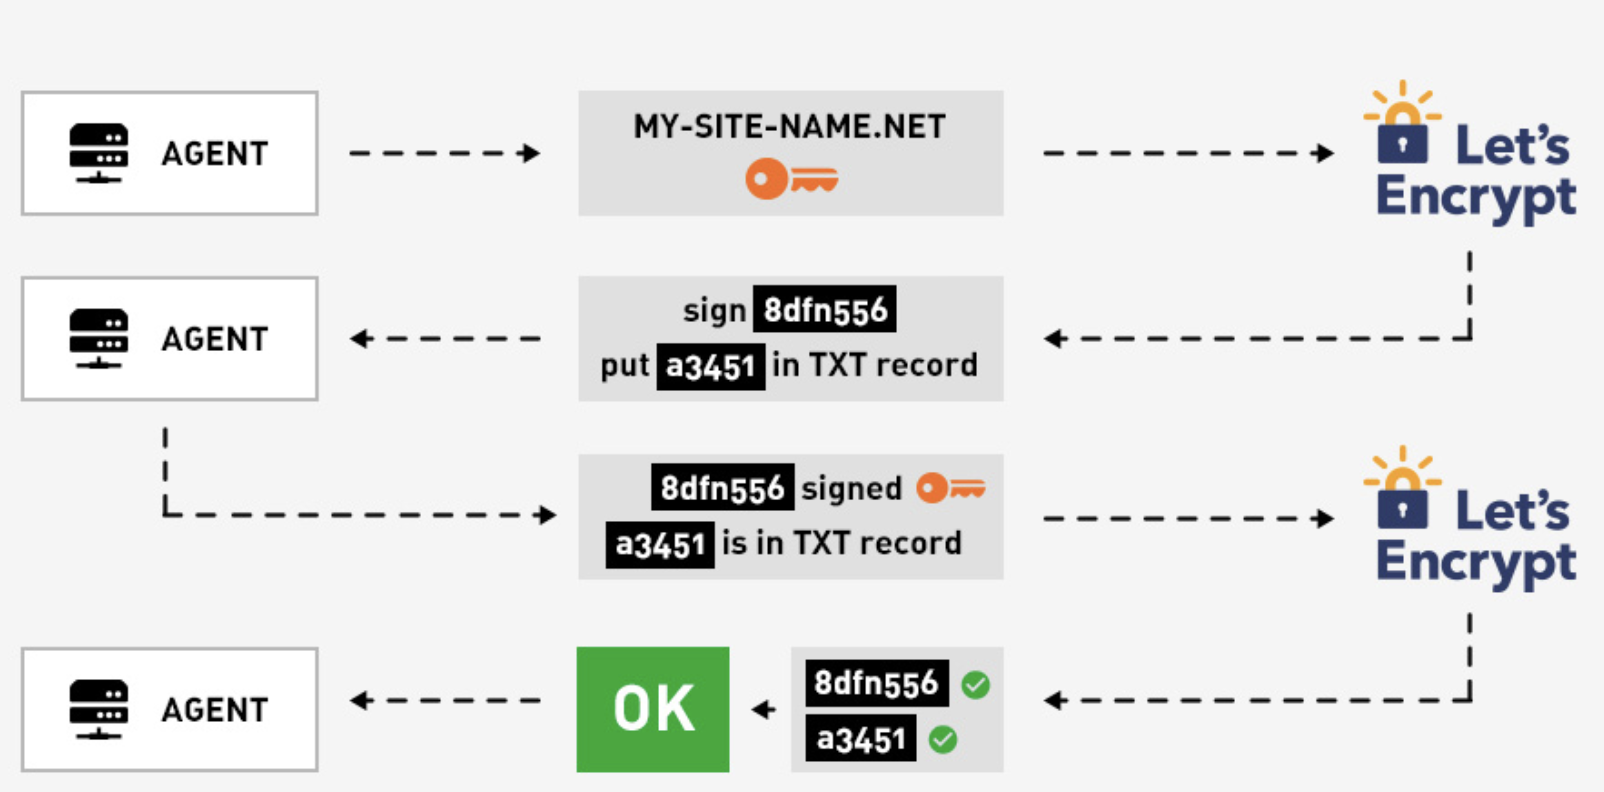
\includegraphics[width=0.35\textwidth]{lets_encrypt}
        \end{center}
    \end{figure}

    \begin{minted}{bash}
sudo apt install -y certbot python3-certbot-nginx
sudo ufw allow 80/tcp 443/tcp
sudo certbot --nginx -d api.example.com
    \end{minted}

    Certbot validates the domain (places a file under \texttt{/.well-known/}, lets Let's Encrypt fetch it), installs the cert, edits the Nginx config to add the \texttt{listen 443 ssl;} block, sets up auto-renewal.
\end{frame}

\begin{frame}[fragile]{All together}
    Visit \texttt{https://api.example.com} in a browser. Padlock icon, certificate issued by Let's Encrypt.
    HTTP requests redirect to HTTPS automatically.

    \vspace{0.5em}
    Renewal runs through a systemd timer Certbot installed.
    Dry-run to confirm:

\begin{minted}{bash}
sudo certbot renew --dry-run
\end{minted}

\end{frame}


\section{Exercise}

\begin{frame}{Deploy your server to the cloud}
    Take the image from the Module B.3 exercise. Bring it up on a cloud VM.
    Point the A.2 client at it.

    \begin{block}{Outline}
        \begin{enumerate}
            \item Pick a provider. Free tier (AWS/GCP/Azure trial credits) or cheap small VM (Hetzner, DO, Vultr)
            \item Create a small VM and setup the basic runtime
            \item Pull your image and run it, then point the A.2 client at \texttt{http://<VM\_IP>:<PORT>} and run a few requests
        \end{enumerate}
    \end{block}
\end{frame}

\begin{frame}{Extensions}
    \begin{enumerate}
        \item Get a free domain on DuckDNS, point an A record at the VM
        \item Install Nginx, configure it as a reverse proxy on port 80. Confirm the API still works through \texttt{http://<your-domain>}
        \item Get a HTTPS certificate with Certbot and Let's Encrypt
        \item Update the A.2 client to use the HTTPS URL, confirm requests still go through
    \end{enumerate}
\end{frame}

% TODO: Add a "What you should walk away with" slide


\appendix

\begin{frame}[plain,noframenumbering]
\begin{center}
{\large Thank you!}
\vspace{1cm}
\\[0.5em]
{\small \faEnvelope\ \href{mailto:lyan@cs.aau.dk}{lyan@cs.aau.dk} \\
\faGlobe\ \href{https://www.yanlincs.com}{www.yanlincs.com}}
\end{center}
\end{frame}

\end{document}
